\section{Pushing our Luck above Cuckoo's Nest}
\margininbox{Push Your Luck}{
     \begin{itemize}
    \item Rhys Tyers
    \item Tanguy Racine
    \end{itemize}}{\explo}
    
We'd overslept a lot I decided as I saw that it was already past ten o'clock. It did not surprise me, since we'd only come back from Meridian Way just before midnight. Then we'd collapsed into bed.
 In the darkness of the tent I sat upright in the snug sleeping bag, furry hat on. My breath turned to a silvery mist by the light of my headtorch. The fairy lights had dimmed so much I could hardly make them out. I left the comfort and warmth of the Nitestar 450, put on the largest crocks I could find, and lit the church candles. One, two, three dancing lights.

 \begin{marginfigure}
\checkoddpage \ifoddpage \forcerectofloat \else \forceversofloat \fi
\centering
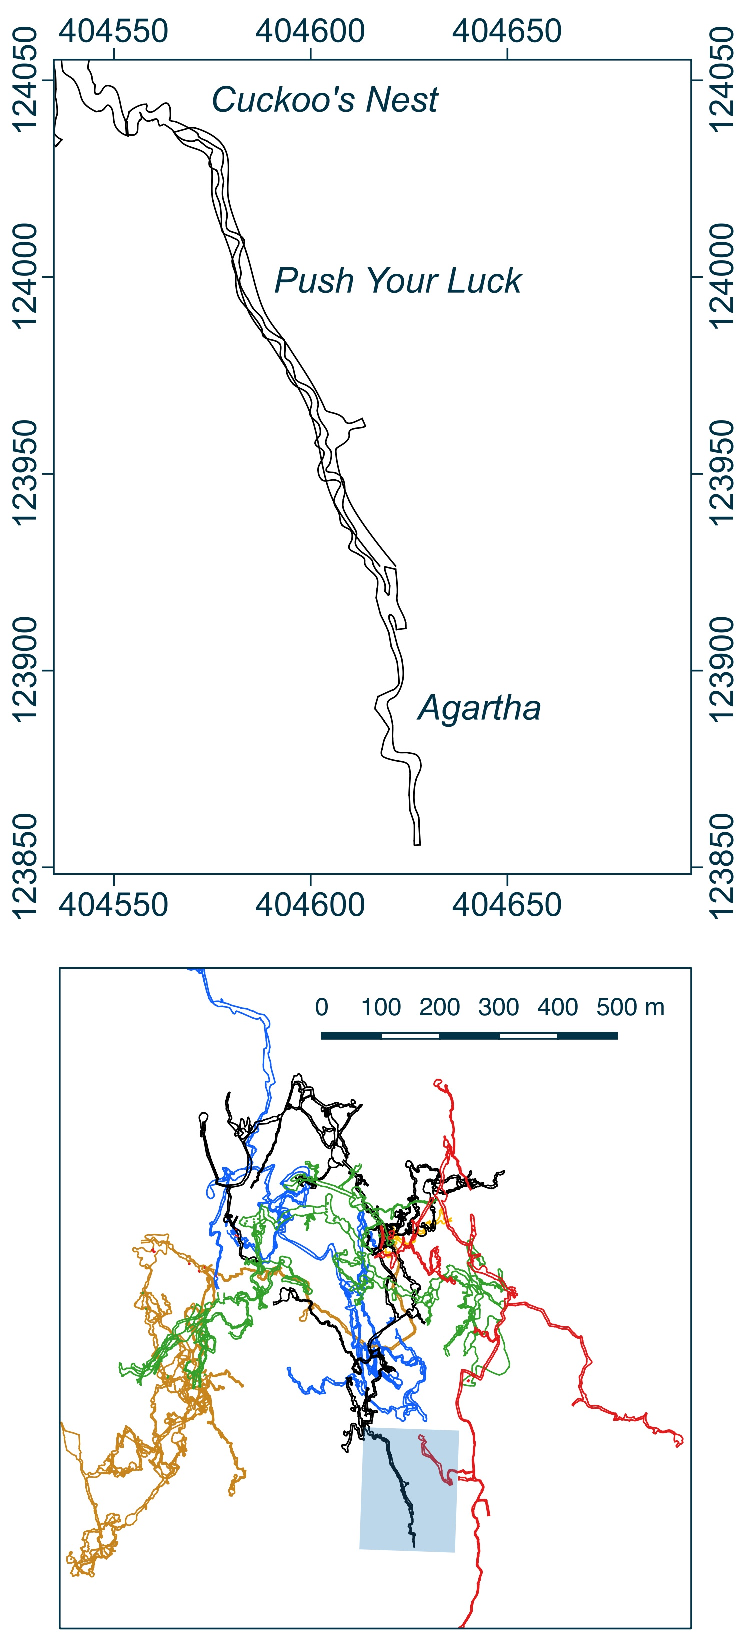
\includegraphics[width= \linewidth]{images/little_insets/push_your_luck_inset.pdf}
 \caption*{Plan view of the \protect\passage[extensions]{Cuckoo's Nest} extensions, Slovenian National Grid ESPG 3794}
 \label{push your luck inset}
\end{marginfigure}

`Where are we going to push then' I asked Rhys, whilst tucking into a rich soupy couscous mix.
`I know of a lead Clare pushed in 2013, up \passage{Cuckoo's Nest}' he replied.
`I've never been down that way. How do you get to the passage? Is it past the traverse at the top of \passage{Big Rock Candy Mountain}'
`Yeah, that's it, you traverse and then drop into a chamber. There'll be a rope on your right, the one from \passage{Euphrates}. It's a grim bit of cave, which is why no one's ever gone back to retrieve the rope after surveying. It connects back to Xanadon't and the hole in \passage{Friendship Gallery}.'
`Fascinating, so fairly close to camp then. Shall we?'
`I'm going to put our call out as 7pm then'.

Half an hour later, we left camp, along \passage{Friendship Gallery}, towards the head of \passage{Big Rock}. There we kept to the right, traversed on the muddy pitch head, until a short succession of small hangs brought us into a chamber overlooking the massive drop. After a small climb down, we followed a sinuous muddy rift until we had to climb up again unsing a greasy in situ rope. From then on, the rumble of flowing water could be heard distinctly, and we soon came upon a fork in the passage, with the way to \passage{Straight Jacket} and \passage{Rejuvenation Rift} to our right. The way on to the end of \passage{Cuckoo's Nest} was to the left, with the passage descending slightly until we reached the water at the bottom of the rift.

Past a few meanders, the rift widened to an oval shape and a cascade three metres high draped the far wall. A PSS was left underneath a egg like pure white limeston cobble: \passage{Cuckoo's Nest} station 3. Rhys and I contemplated the pushing front. The only viable way on was up, and could be reached by bridging our way up, away from the water. Several ledges were seen to protrude, giving steady footholds about two and a half metres from the floor. Feet and back against the scalloped walls, Rhys  climbed up gracefully and I followed.

At the first ledge I started removing the majority of loose rocks I could reach, while Rhys gained more height. Ledge by ledge we climbed until we reached the top of the traverse, dry, muddy, and loose. There we steadily traversed in the upstream direction, until we dropped into the streamway again. We were faced with a similar second climb. Further traverse enabled us to gain the top of third cascade, after which we continued almost a stream level on a meandering rift heading steadily southward.

\begin{figure}[t!]
\checkoddpage \ifoddpage \forcerectofloat \else \forceversofloat \fi
\centering
\frame{\includegraphics[width=\textwidth]{"images/2015/tanguy-push-2015/push_your_luck".png}}
\caption{The plan view of the \emph{Push your Luck} streamway, an active undergound stream which journeys northward all the way to \emph{Highway 32} \pen{Tanguy Racine, underground logbook}}
\label{}
\end{figure}


 \begin{marginfigure}
	\checkoddpage \ifoddpage \forcerectofloat \else \forceversofloat \fi
	\centering
\vspace{-100pt}
	\frame{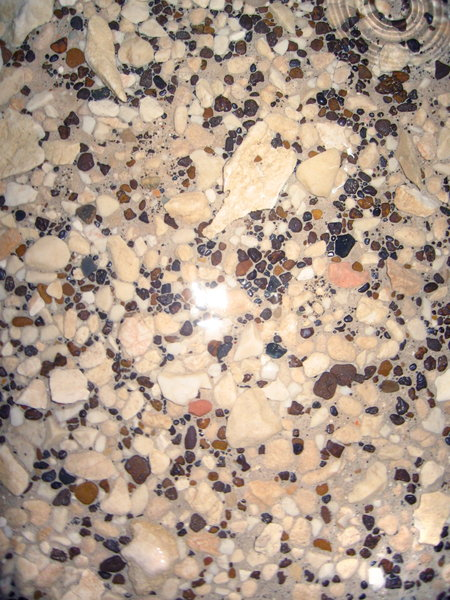
\includegraphics[width=\linewidth]{images/2015/tanguy-push-2015/pebbles_in_alchemy_jana_carga.jpg}}
	\caption{Pebbles similar to those found in \protect\passage{Push Your Luck} streamway can also be seen at the bottom of \protect\passage{Alchemy} pitch in the entrance series of \protect\passage{Vrtnarija} \pic{Jana \v{C}arga}}
	\label{push your luck pebbles}
\end{marginfigure}

Our progress was not hampered by any further climbs or constrictions, and soon I lost count of the twists and turns. We arrived a boulder collapse. Navigating our way in the vertical maze we eventually reached the roof again, but to our surprise, a flat out crawl lead off back in the opposite direction. Instead of following it we negotiated the way past the collapse, and regained the stream. From then on, the rift enlarged particularly on the occasion of three meanders, where the base was very much wider, the stream lazier and where sediments had deposited on the shelves: granules and small pebbles of white limestone and black haematite. This was a delightful sight, the finest photogenic cave sediments I'd seen on \passage{Mig}!

After the meanders, the rift resumed its course and after a further collapse Rhys and I called it day. This was more than enough rift to survey. Doubling back to the start of the passage to get survey paper and instruments, we tried to gauge the length of our find. With the 350m discovered a day earlier at \passage{Meridian Way}, would we reach the 500m of passage found in one camping trip'


As I took the survey notebook and pencil, I stuffed my gloves inside my oversuit, and we started the survey. After the climbs, we started the meanders. As I sat, writing down the lengths and angles Rhys dictated the gloves fell down to my navel and made a noticeable bulge underneath the suit.
\bignote{`Tanguy, are these your gloves, or are you just happy to see me?'} asked Rhys.
`It's the passage' I answered, and we both had a good laugh.

After fifty or so survey legs, we arrived at the boulder collapse. I ate a chocolate bar while my partner in crime added up the legs. `About 250m in the book, what a lovely tourist trip - that's what you call pushing one's luck'.

\name{Tanguy Racine}
